\documentclass[twocolumn,3p,a4paper,preprint,11pt,margin=2.5cm]{elsarticle}
% \documentclass{article}
\usepackage{graphicx} % Required for inserting images
% \usepackage[margin=2.5cm]{geometry}
\usepackage{amsmath}
\usepackage{makecell} % To allow multiple lines in a table cell
\usepackage{multirow}
\usepackage{booktabs}  % For professional tables
\usepackage{float}  
\usepackage[utf8]{inputenc}
\usepackage{xcolor} % For setting text opacity
\usepackage{tikz} % Package for drawing shapes and lines
\usepackage{multicol}
\usepackage{blindtext}
\usepackage{hyperref}
\usepackage[style=ieee,sorting=ynt]{biblatex} % Set IEEE style
\usepackage{float}
\addbibresource{ref.bib}
\usepackage{titlesec}
\usepackage{enumitem} % For customizing enumeration
\usepackage{caption}
\usepackage{subcaption}



% Customizing the section format
\titleformat{\section}
  {\Large\bfseries} % Set size and boldface for section number and title
  {\thesection}     % Print section number
  {1em}             % Space between the number and the title
  {\Large} 

% Customizing the subsection format
\titleformat{\subsection}
  {\large\bfseries} % Set size and boldface for subsection number and title
  {\thesubsection}  % Print subsection number
  {1em}             % Space between the number and the title
  {\large} 

\title{
\vspace{-20mm} % Adjust vertical space above the top line
    \hrule height 1.5pt \vspace{8mm} % Top line
    \textbf{Unifying Vision-and-Language Tasks via Text Generation}
    \vspace{8mm} % Space between title and bottom line
    \hrule height 1.5pt % Bottom line
    \vspace{3mm} % Adjust space below the bottom line
}
\author{
    \textbf{Jaemin Cho\textsuperscript{\textnormal{1}}\hspace{0.2cm} Jie Lei\hspace{0.2cm} Hao Tan\hspace{0.2cm} Mohit Bansal}\\
UNC Chapel Hill\\
\textcolor[gray]{0.5}{\texttt{\{jmincho, jielei, haotan, mbansal\}@cs.unc.edu}}
}
\date{}
\makeatletter
\long\def\pprintMaketitle{\clearpage
  \thispagestyle{empty}%
  \vskip 2em%
  \def\baselinestretch{1}%
  \begin{center}%
  \def\baselinestretch{1}%
  \@title\par\vskip 1em%
  {\small\@author}\par\vskip 1em%
  {\small\@date}\par\vskip 1em%
  \end{center}%
  \ifvoid\@abstractbox\else\centerline{\begin{minipage}{0.95\textwidth}\unvbox\@abstractbox\end{minipage}}\fi
  \vskip 1.5em}%
\makeatother
\begin{document}


\maketitle

% \begin{abstract}
% Your abstract goes here. It should be a concise summary of your article.
% \end{abstract}



\begin{center}
 \Large{\textbf{Abstract}}\\
\end{center}
Existing methods for vision-and-language learning typically require designing 
task-specific architectures and objectives for each task. For example, a multi-label answer classifier for visual question answering, a region scorer for referring
expression comprehension, and a language decoder for image captioning, etc.To alleviate these hassles, in this work, we propose a unified framework that learns different tasks in a single architecture with the same language modeling objective, i.e., multimodal conditional text generation, where our models learn to generate
labels in text based on the visual and textual inputs. On 7 popular vision-and-language benchmarks, including visual question answering, referring expression comprehension, visual commonsense reasoning, most of which have been previously modeled as discriminative tasks, our generative approach (with a single unified architecture) reaches comparable performance to recent taskspecific state-of-the-art vision-and-language models. Moreover, our generative approach shows better generalization ability on questions that have rare answers. Also, we show that our framework allows multi-task learning in a single architecture with a single set of parameters, achieving similar performance to separately optimized single-task models. Our code is publicly available at: \href{https://github.com/j-min/VL-T5}{https://github.com/j-min/VL-T5}

\section{\Large{Introduction}}
\vspace{0.3 cm}
\begin{figure}[H]
    \centering
    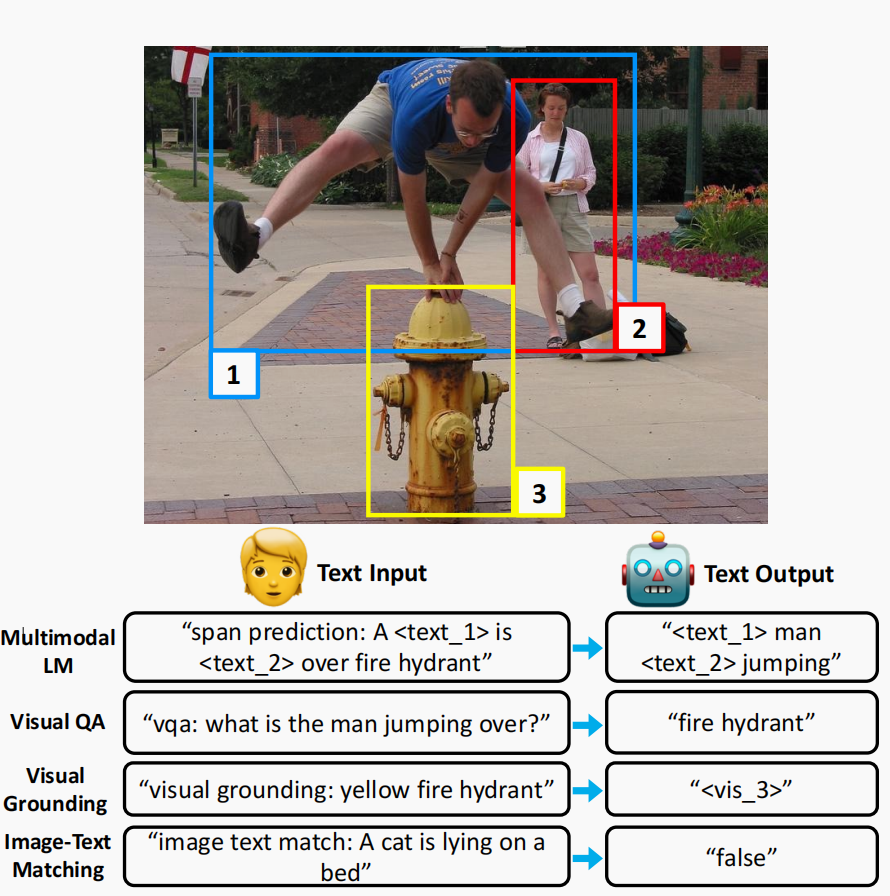
\includegraphics[width=0.8\linewidth]{image/Image1.png}
    \caption{Our unified framework for learning vision-and-language
tasks. While existing methods require designing task-specific architectures for different tasks, our framework unifies them together
as generating text labels conditioned on multimodal inputs}
    \label{fig:enter-label}
\end{figure}
Recent vision-and-language transformers have made great strides by using a pretraining approach which has led to impressive results in tasks such as visual question answering and referring expression comprehension. Still, these models usually need specific setups for each task, even when they share similar reasoning skills.\\[2pt]
To tackle this issue, the authors suggest a unified framework that relies on text generation. They’ve extended powerful pretrained models like T5 and BART by adding visual abilities and call these enhanced versions VL-T5 and VL-BART.\\[2pt]
This new method allows for multiple tasks through one architecture without needing more parameters. Experiments reveal that this unified approach matches the performance of top models across several benchmarks which also shows better generalization, especially in situations with rare answers.\\
\section{\Large{Related Works}}
\vspace{0.3 cm}
\textbf{Vision-and-Language pretraining:}\\
Large-scale language pretraining with transformers (\cite{vaswani};
\cite{MingWeiChang}; \cite{YinhanLiu}) have achieved
remarkable success for many natural language understanding tasks(\cite{RowanZellers})  Following this success, image+text pretraining models (\cite{ZhichengHuang})  and video+text pretraining models (\cite{ChenSun}) have also shown to perform better than previous non-pretraining approaches (\cite{Anderson}) in a wide range
of discriminative (\cite{Hudson}) and generative tasks (\cite{XinleiChen}). In this work, we focus on
image+text tasks. While existing image+text models mostly
use task-specific architectures and objectives, we seek to
design a unified framework across different tasks.\\
\section{\Large{Model}}
\vspace{0.3 cm}
We propose a new framework that unifies vision-and language problems as multimodal conditional text generation. We introduce VL-T5 and VL-BART based on two pretrained transformer language models: T5Base and BARTBase. Specifically, we extend their text encoders to multimodal encoders by incorporating image region embeddings as additional input. The overall architecture of our framework is shown in Fig. 2. Since the architecture differences between VL-T5 and VL-BART are minor, we use VL-T5 as an example to illustrate our framework in detail in the rest of this section.

\subsection{Visual Embeddings}
\vspace{0.3 cm}
We represent an input image v with n=36 object regions from a Faster R-CNN trained on Visual Genome. As shown in Fig. \ref{fig:embedding}, each image region is encoded as a sum of four types of features: 
\noindent % Remove indentation
\begin{enumerate}[label=(\roman*)] % Roman numerals, inline list with semicolon separator
    \item RoI (Region of Interest) object features
    \item RoI bounding box coordinates
    \item image IDs $\in \{1, 2\}$
    \item region IDs $\in \{1, \dots, n\}$
\end{enumerate}.
RoI features and bounding box
coordinates are encoded with a linear layer, while image ids
and region ids are encoded with learned embeddings (Devlin et al., 2019). Image ids are used to discriminate regions
from different images, and is used when multiple images
are given to the model (i.e., in NLVR2 (Suhr et al., 2019),
models take two input images). The final visual embeddings
are denoted as $e^{v} = \{e_{1}^{v}, \dots ,e_{n}^{v}\}$
\subsection{Encoder-Decoder Architecture}
We use\textit{ transformer encoder-decoder architecture} \cite{vaswani} to encode visual and text inputs and generate label text. Our bidirectional multi modal encoder is a stack of $m$ transformer blocks, consisting of a self-attention layer and a fully-connected layer with residual connections. Our decoder is another stack of $m$ transformer blocks similar to the multi modal encoder, where each block has an additional cross-attention layer. As shown in figure \ref{fig:embedding}, the encoder takes the concatenation of text and visual embedding as input and outputs their contextualized joint representations 
$$ h = \{h^x_1, \dots, h^x_{|x|}, h^v_1, \dots, h^v_n\} = \text{Enc}(e^x, e^v). $$ 
\begin{figure*}[tp] % Use figure* to span both columns
    \centering
    % First subfigure
    \begin{subfigure}{0.45\textwidth} % 45% of total page width for the first image
        \centering
        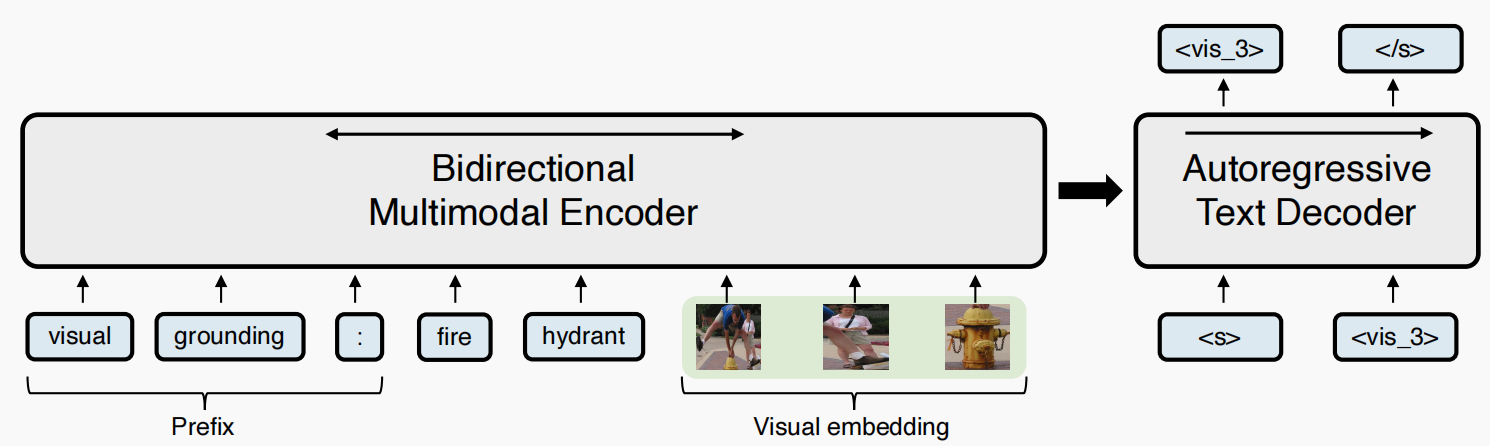
\includegraphics[height=8cm,width=\textwidth]{image/image2.png}
        \caption{Our vision-and-language framework}
        \label{fig:framework}
    \end{subfigure}
    % Vertical dashed line using TikZ
    \begin{tikzpicture}
        \draw[dashed] (0,-4) -- (0,4); % Adjust height for the dashed line
    \end{tikzpicture}
    \hfill
    % Second subfigure
    \begin{subfigure}{0.45\textwidth} % 45% of total page width for the second image
        \centering
        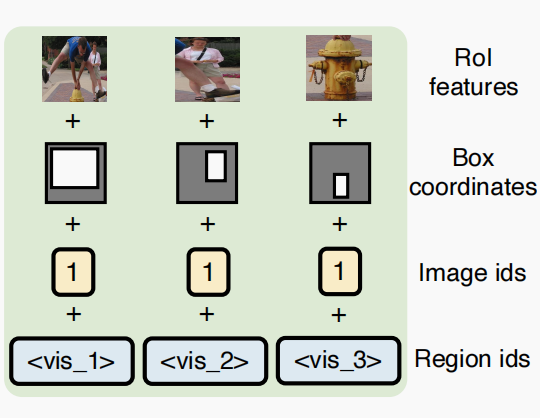
\includegraphics[width=\textwidth]{image/image3.png}
        \caption{Visual embedding}
        \label{fig:embedding}
    \end{subfigure}
    % Overall figure caption
    \caption{An illustration of our VL-T5 and VL-BART architectures for visual grounding task. Instead of task-specific architectures, our
models use text prefixes to adapt to different tasks. The green block in (a) refers to visual embeddings. (b) shows the components of visual
embedding. Note that we reuse the text embeddings of visual sentinel tokens (ex. <vis 3>) as region id embeddings, which allows our
models to tackle many discriminative vision-language tasks as text generation, including visual grounding.}
    \label{fig:combined}
\end{figure*}

Then the decoder iteratively attends to previously generated tokens $y_{<j}$ (via self-attention) and the encoder outputs $h$ (via cross-attention), then predicts the probability of future text tokens
$$ P_{\theta}(y_j | y_{<j}, x, v) = \text{Dec}(y_{<j}, h). $$
We suggest readers to check \cite{MingWeiChang} \cite{XinleiChen} for more details of our backbone models. For both pretraining (Sec. 4) and downstream tasks (Sec. 5), we train our model parameters $\theta$ by minimizing the negative log-likelihood of label text $y$ tokens given input text $x$ and image $v$:
\begin{equation}
     \mathcal{L}^{GEN}_{\theta} = - \frac{1}{|y|} \sum_{j=1}^{|y|} \log P_{\theta}(y_j | y_{<j}, x, v) \label{eq:first}
\end{equation}

\subsection{Task-Specific Methods vs. Our Unified Framework}
\begin{figure}[H]
    \centering
    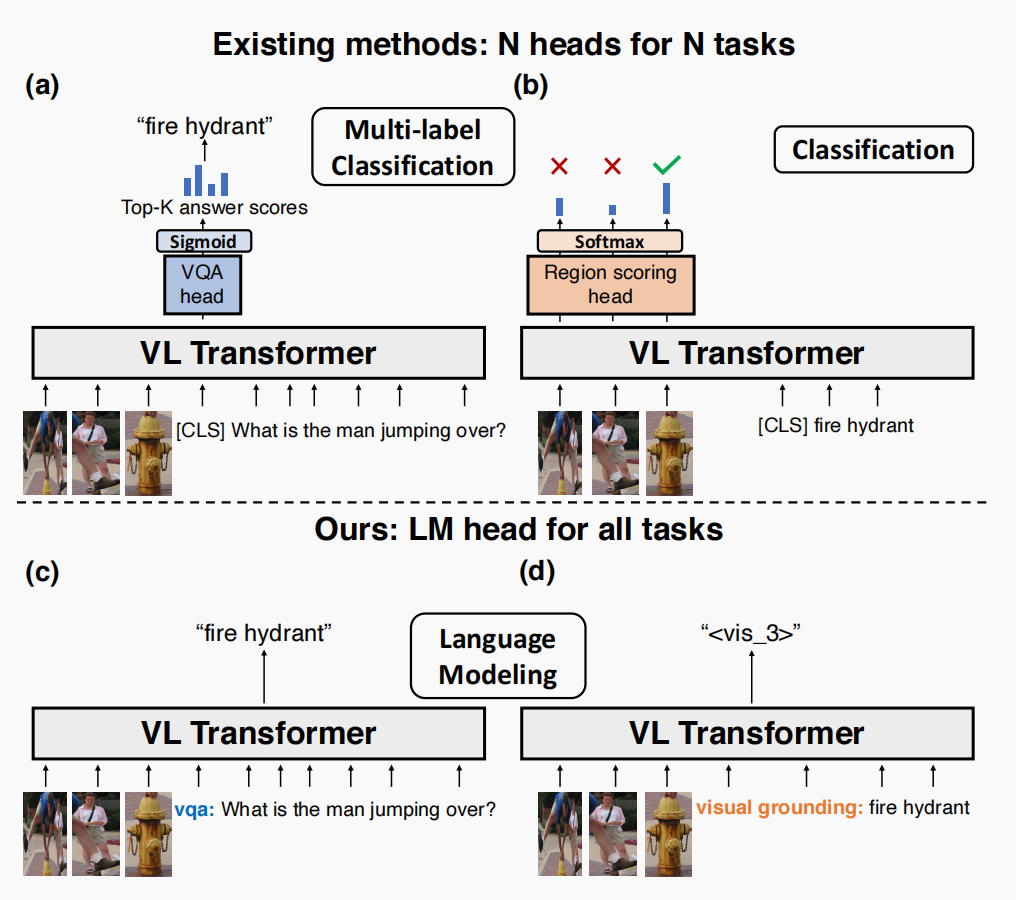
\includegraphics[width=1\columnwidth]{image/image4.png}
    \caption{Comparison between existing methods and our frame-work on visual question answering and referring expression comprehension (visual grounding) tasks. While existing methods use
task-specific architectures and objectives, our models use the same
language modeling architecture and maximum likelihood estimation on label text for all tasks.}
    \label{fig:comparison}
\end{figure}

We compare our unified framework with existing vision-and-language transformers on two popular tasks: visual question
answering (\cite{Anderson}) and referring expression
comprehension (\cite{Hudson}).\\[0.4 cm]
\textbf{Visual question answering }requires a model to answer
a question to a given context image. As shown in figure \ref{fig:comparison}, existing methods (\cite{Anderson}; \cite{XinleiChen})  typically introduce a multi-layer perception (MLP) multi-label classifier head on
top of $ h_{[cls]}^x $ , which is trained together with the transformer backbone through a binary cross-entropy loss, and weighted with VQA score\\[0.2 cm]
$\mathcal{L}_{\theta}^{VQA} = -\\
\sum_{k=1}^{K}\,score(a^{k},x,v) \log P_{\theta}^{VQA}(correct|a^{k}, x, v).$\\[0.4 cm]
\textbf{Referring expression comprehension }requires models to
localize a target region in an image that is described by
a given referring expression. Previous methods tackle
this task as multi-class (\cite{XinleiChen}) or binary (\cite{MingWeiChang}) classification over image regions. For example, UNITER (\cite{XinleiChen}) introduces an MLP region
scoring head on top of the output representations of regions, as shown in figure \ref{fig:comparison}. This region scoring head is jointly trained with the encoder by minimizing negative log-likelihood of target region\\[0.4 cm]
$ r^{*}: \mathcal{L}_{\theta}^{REF} = - \log P_{\theta}^{REF}(r^{*}|x,v).$
In contrast to existing methods that develop task-specific
architectures and objectives (e.g., the equations above), our
unified framework is free from extra model designs for new
tasks. As shown in Figure \ref{fig:comparison} and Table \ref{tab:comparison2}, we formulate
the task labels to corresponding text, and we learn these different tasks by predicting label text with the same language modeling objective Equation~\ref{eq:first}.

\begin{table}[H]
\centering
\resizebox{\columnwidth}{!}{%
\begin{tabular}{lccc}
\hline
\textbf{Method}       & \textbf{In-domain} & \textbf{Out-of-domain} & \textbf{Overall} \\ \hline
\multicolumn{4}{l}{\textbf{Discriminative}} \\
\textbf{UNITER\textsubscript{Base}} & 74.4 & 10.0 & 70.5 \\
\textbf{VL-T5}         & 70.2 & 7.1  & 66.4 \\
\textbf{VL-BART}       & 69.4 & 7.0  & 65.7 \\
\multicolumn{4}{l}{\textbf{Generative}} \\
\textbf{VL-T5}         & 71.4 & 13.1 & 67.9 \\
\textbf{VL-BART}       & 72.1 & 13.2 & 68.6 \\ \hline
\end{tabular}
}
\caption{VQA Karpathy-test split accuracy using generative and
discriminative methods. We break down the questions into two
subsets in terms of whether the best-scoring answer $a^{*}$
for each question is included in the top-K answer candidates $A^{topk}$. In domain: $a^{*} \in A^{topk}$, Out-of-domain: $a^{*} \notin A^{topk} $ }
\label{tab:comparison}
\end{table}

\section{\Large{Downstream Tasks and Results}}
In this section, we compare our generative architectures VL-T5 and VL-BART on a diverse set of 7 downstream tasks
(details in Appendix) with existing vision-and-language pre-trained transformers.\\[0.4 cm]
\subsection{ Visual Question Answering: VQA and GQA}
The visual question answering task requires models to answer a question to a given context image.\\[0.4 cm]
\textbf{Generative vs. Discriminative model:} Modern approaches are discriminative models, where they tackle visual question answering tasks as multi-label classification over a predefined set of answer
candidates. This strategy achieves strong performance but
not generalizes to real-world open-ended scenarios. To quantitatively compare the existing discriminative approaches
and our generative approach, we break down VQA questions into in-domain and out-of-domain questions, in terms of whether the best answer $a^*$ for each question is included in the top-K (K=3, 129) answer candidates $A^{TopK}$. After this split, the in-domain subset contains 24,722 questions, and 
% % Create the table
% \clearpage  % Forces a new page and flushes floats
\vspace*{-10pt}
\begin{table*}[tp]
\centering
\caption{Input-output formats for pretraining (Sec. 4) and downstream tasks (Sec. 5).}
\label{tab:comparison2}
\resizebox{\textwidth}{!}{%
\begin{tabular}{l l l l}
\hline
\textbf{Tasks} & \textbf{Input image} & \textbf{Input text} & \textbf{Target text} \\ 
\hline
\makecell[l]{\textbf{Pretraining text (Sec-4)}\\Multimodal LM (VL-T5)\\ Multimodal LM (VL-BART)\\ " Visual\\ question answering\\ Image-text matching\\ Visual grounding\\ Grounded captioning} &
\multirow{2}{*}{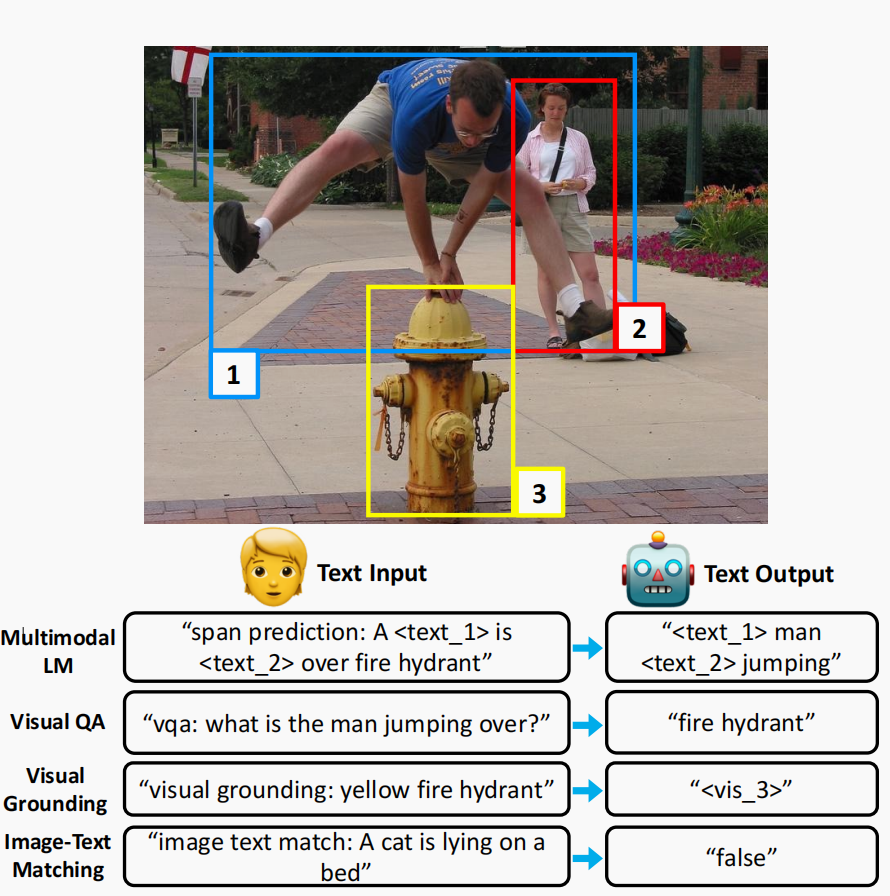
\includegraphics[width=0.8\columnwidth]{image/Image1.png}} &
\makecell[l]{span prediction: A $\langle text_1 \rangle $ is $\langle text_2 \rangle $\\ over a fire hydrant.\\ denoise: A $\langle mask \rangle $ is $\langle mask \rangle $\\ over a fire hydrant.\\ vqa: what is the color\\ of the man's shirt?\\
image text match:\\ A man with blue shirt is\\ jumping over fire hydrant.\\
visual grounding:\\ yellow fire hydrant\\ caption region: $\langle vis_3 \rangle $} &
\makecell[l]{$\langle text_1 \rangle $ man $\langle text_2 \rangle $ jumping\\ A man is jumping\\ over a fire hydrant\\
blue true $\langle vis_3 \rangle $\\
yellow fire hydrant}\\
\cline{1-1}\cline{3-4}\\
\makecell[l]{\textbf{Downstream tasks (Sec. 5)} \\ 
VQA \\
GQA \\
\textsuperscript{b}NLVR\textsuperscript{2} \\
VCR Q$\rightarrow$A \\
VCR QA$\rightarrow$R \\
RefCOCOg \\
COCO captioning \\
COCO captioning (w/ object tags) \\
Multi30K En-De translation} & &
\makecell[l]{vqa: [2]\\
gga: [2]\\
nIvr: [text ]\\
vcr qa: question [Q] answer: [A]\\
vcr qar: question [Q] answer: [A] rationale: [R]\\ visual grounding: [referring expression]\\
caption:\\
caption with tags: [Tagl Tag2 \dots] \\translate English to German: [English text]} &
\makecell[l]{[A]\\
[A]\\
true/false\\
true/false \\
true/false\\
[region id]\\[caption] \\
[caption]\\[German text]
}\\
\hline
\end{tabular}
}
\end{table*}
the out-of-domain subset contains 1,558 questions. Table \ref{tab:comparison} shows the performance. For discriminative baselines, we introduce a sigmoid MLP classifier on top of the decoder representation of the start-of-sequence token $\langle s \rangle$, following \textbf{LXMERT} and \textbf{UNITER}. Comparing models with the same backbone, we notice that the generative models improve upon the discriminative baselines across all subsets. This improvement is more significant on the out-of-domain subset, where the generative \textbf{VL-T5} and \textbf{VL-BART} achieve 6 and 6.2 points improvement over their discriminative counterparts, showing the effectiveness of using generative modeling. Compared to the strong discriminative baseline \textbf{UNITER\textsubscript{Base}} (pretrained with 4M extra images), our generative models still show comparable overall performance while significantly outperforming it on the out-of-domain subset (about 3 points).

\subsection{Visual Commonsense Reasoning: VCR}
Visual Commonsense Reasoning (VCR) (\cite{ZhichengHuang}) is a multiple-choice question answering task that
requires commonsense reasoning beyond object or action
recognition. Each VCR question (Q) has 4 answers (A)
and 4 rationales (R), and it can be decomposed into two
multiple choice sub-tasks: question answering ($Q \rightarrow A$), and answer justification ($QA \rightarrow A$). The overall task ($Q \rightarrow AR$) requires a model to not only select the correct answer to the question, but also the correct rationale for choosing the answer. Similar to that leverages language model for document ranking, we concatenate context (image+question) with each candidate choice, and let our models generate “true” for the correct choice and generate “false” otherwise, as shown in table \ref{tab:comparison2}, During inference, we use $\dfrac{P(true)}{P(true)+P(false)}$ to rank the choices and select the one with the highest score.\\[0.4 cm]
\section{\Large{Conclusion}}
In this work, we proposed VL-T5 and VL-BART which
tackle vision-and-language tasks with a unified text generation objective. Experiments show VL-T5 and VL-BART
can achieve comparable performance with state-of-the-art
vision-and-language transformers on diverse vision-and-language tasks without hand-crafted architectures and objectives. Especially, we demonstrate our generative approach
is better suited for open-ended visual question answering.
In addition, we also showed it is possible to train seven different tasks simultaneously using a single architecture with
single parameters without not losing much performance. It
would be an interesting future work to further explore this
direction by adding even more tasks.

% \clearpage  % Forces a new page and flushes floats (like tables and figures) before moving on

\printbibliography

\end{document}
